\documentclass[11pt,a4paper]{article}

% ============================================================
% Shared FSFC--PRIO--VIEWS preamble for the views-lab00
% research notes triptych. Adapted from the FAO pre-release note
% 05 preamble (papers/_assets/style adapted from
% fao_02_pre_release_note_05/main.tex).
%
% Each note's main.tex should include this file with:
%   % ============================================================
% Shared FSFC--PRIO--VIEWS preamble for the views-lab00
% research notes triptych. Adapted from the FAO pre-release note
% 05 preamble (papers/_assets/style adapted from
% fao_02_pre_release_note_05/main.tex).
%
% Each note's main.tex should include this file with:
%   % ============================================================
% Shared FSFC--PRIO--VIEWS preamble for the views-lab00
% research notes triptych. Adapted from the FAO pre-release note
% 05 preamble (papers/_assets/style adapted from
% fao_02_pre_release_note_05/main.tex).
%
% Each note's main.tex should include this file with:
%   \input{../_assets/preamble}
% ============================================================

% LANGUAGE & ENCODING
\usepackage[english]{babel}
\usepackage[utf8]{inputenc}

% TYPOGRAPHY & SPACING
\usepackage{microtype}
\usepackage[onehalfspacing]{setspace}
\usepackage{parskip}
\setlength{\footnotesep}{0.7\baselineskip}
\usepackage[hang,flushmargin]{footmisc}

% PAGE LAYOUT
\usepackage[a4paper,margin=1in]{geometry}
\usepackage{fancyhdr}
\pagestyle{fancy}
\fancyhf{}
\lhead{Maase et al.}
\rhead{\today}
\lfoot{PRIO --- VIEWS}
\rfoot{\thepage}
\renewcommand{\footrulewidth}{0.8pt}

% GRAPHICS & TABLES
\usepackage{graphicx}
\usepackage{booktabs}
\usepackage{makecell}
\usepackage[section]{placeins}
\usepackage[table]{xcolor}

% MATH & SYMBOLS
\usepackage{amsmath,amssymb}

% CITATION & QUOTING
\usepackage{csquotes}
\usepackage{natbib}

% HYPERLINKS
\usepackage[hidelinks]{hyperref}

% NOTES
\usepackage[colorinlistoftodos]{todonotes}

% TITLE
\usepackage{titling}
\pretitle{\vspace{2em}\centering\Huge\bfseries}
\posttitle{\par\vspace{1em}}
\preauthor{\centering\large}
\postauthor{\par\vspace{0.5em}}
\predate{\centering\small}
\postdate{\par\vspace{2em}}

\author{von der Maase, Dornin Pinheiro \& Häffner}
\date{\today}

% ============================================================

% LANGUAGE & ENCODING
\usepackage[english]{babel}
\usepackage[utf8]{inputenc}

% TYPOGRAPHY & SPACING
\usepackage{microtype}
\usepackage[onehalfspacing]{setspace}
\usepackage{parskip}
\setlength{\footnotesep}{0.7\baselineskip}
\usepackage[hang,flushmargin]{footmisc}

% PAGE LAYOUT
\usepackage[a4paper,margin=1in]{geometry}
\usepackage{fancyhdr}
\pagestyle{fancy}
\fancyhf{}
\lhead{Maase et al.}
\rhead{\today}
\lfoot{PRIO --- VIEWS}
\rfoot{\thepage}
\renewcommand{\footrulewidth}{0.8pt}

% GRAPHICS & TABLES
\usepackage{graphicx}
\usepackage{booktabs}
\usepackage{makecell}
\usepackage[section]{placeins}
\usepackage[table]{xcolor}

% MATH & SYMBOLS
\usepackage{amsmath,amssymb}

% CITATION & QUOTING
\usepackage{csquotes}
\usepackage{natbib}

% HYPERLINKS
\usepackage[hidelinks]{hyperref}

% NOTES
\usepackage[colorinlistoftodos]{todonotes}

% TITLE
\usepackage{titling}
\pretitle{\vspace{2em}\centering\Huge\bfseries}
\posttitle{\par\vspace{1em}}
\preauthor{\centering\large}
\postauthor{\par\vspace{0.5em}}
\predate{\centering\small}
\postdate{\par\vspace{2em}}

\author{von der Maase, Dornin Pinheiro \& Häffner}
\date{\today}

% ============================================================

% LANGUAGE & ENCODING
\usepackage[english]{babel}
\usepackage[utf8]{inputenc}

% TYPOGRAPHY & SPACING
\usepackage{microtype}
\usepackage[onehalfspacing]{setspace}
\usepackage{parskip}
\setlength{\footnotesep}{0.7\baselineskip}
\usepackage[hang,flushmargin]{footmisc}

% PAGE LAYOUT
\usepackage[a4paper,margin=1in]{geometry}
\usepackage{fancyhdr}
\pagestyle{fancy}
\fancyhf{}
\lhead{Maase et al.}
\rhead{\today}
\lfoot{PRIO --- VIEWS}
\rfoot{\thepage}
\renewcommand{\footrulewidth}{0.8pt}

% GRAPHICS & TABLES
\usepackage{graphicx}
\usepackage{booktabs}
\usepackage{makecell}
\usepackage[section]{placeins}
\usepackage[table]{xcolor}

% MATH & SYMBOLS
\usepackage{amsmath,amssymb}

% CITATION & QUOTING
\usepackage{csquotes}
\usepackage{natbib}

% HYPERLINKS
\usepackage[hidelinks]{hyperref}

% NOTES
\usepackage[colorinlistoftodos]{todonotes}

% TITLE
\usepackage{titling}
\pretitle{\vspace{2em}\centering\Huge\bfseries}
\posttitle{\par\vspace{1em}}
\preauthor{\centering\large}
\postauthor{\par\vspace{0.5em}}
\predate{\centering\small}
\postdate{\par\vspace{2em}}

\author{von der Maase, Dornin Pinheiro \& Häffner}
\date{\today}


\title{Forecast Evaluation with Observational Uncertainty:\\ A Cram\'er-Distance Perspective}

\begin{document}

\maketitle

\begin{abstract}
\noindent Armed-conflict fatality counts are uncertain. UCDP data---the standard source for conflict forecasting---systematically underreport deaths, with estimated underreporting exceeding 100\% for low-fatality events---meaning the true count may be more than twice the recorded figure \citep{vesco2026uncertainty}. As the field moves from point-estimate predictions toward full predictive distributions \citep{hegre2025prediction}, the question of how to evaluate these distributions becomes critical. The dominant evaluation metric---the Continuous Ranked Probability Score (CRPS)---assumes the observed fatality count is exact. This creates a bias in model selection: CRPS rewards forecasts that concentrate on the reported number over forecasts that honestly represent the uncertainty around it. I show that replacing this assumption with a distribution reflecting what is actually known about the true value yields a well-established metric---the Cram\'er distance, which is simply the standard CRPS generalised from a single observed value to an uncertain observation---that reduces to standard CRPS when observations are precise. I provide three practical recipes for building the observation distribution from sources available to conflict researchers: from UCDP quality bounds, from the empirically grounded uncertainty model of \citet{vesco2026uncertainty}, and from a calibrated parametric default. On 19{,}397 UCDP cell-months, the reformulation reverses the model ranking in 39\% of cases; on operational predictions from HydraNet \citep{VonDerMaase2025hydranet}, a spatio-temporal deep-learning model for conflict forecasting, 99.4\% of cases where the standard metric favours overconfidence are reversed. The metric's reliability depends on the quality of the observation distribution; I characterise the conditions under which mis-specification introduces bias and verify consistency numerically across three distributional families.
\end{abstract}

\paragraph{Significance.}
Forecast competitions and model selection procedures that use CRPS as their ranking metric---such as the 2023/24 VIEWS prediction challenge \citep{hegre2025prediction}---implicitly assume observations are exact. When this assumption is violated, competition rankings can systematically favour overconfident models. I show that accounting for observational uncertainty in forecast evaluation changes which forecast version is judged best, and demonstrate this on both synthetic and operational conflict forecasts (\S5). The argument applies to any domain where observations carry non-trivial uncertainty \citep{bessac2021forecast}.

\section{Introduction}
Armed-conflict fatality counts are derived from media reports, witness accounts, and analyst judgement; the reported value is a noisy estimate of an underlying truth that no single source observes exactly. UCDP---a standard source for conflict forecasting---explicitly provides low/best/high uncertainty bounds per event \citep{ucdp_codebook}, and estimated underreporting exceeds 100\% for low-fatality events \citep{vesco2026uncertainty}. As the field moves toward full predictive distributions---for model ranking, ensemble construction, and operational deployment \citep{hegre2025prediction}---the question of how to evaluate these distributions against uncertain observations becomes critical.

The leading proper scoring rule for distributional forecasts is the Continuous Ranked Probability Score \citep[CRPS;][]{matheson1976scoring,hersbach2000decomposition}. It measures how well a forecast distribution matches an observation: the closer the forecast's cumulative distribution function (CDF) $F_\text{pred}$ is to the observation, the lower the score:
%
\begin{equation}
    \text{CRPS}(F_\text{pred}, y) = \int_{-\infty}^{\infty} \bigl( F_\text{pred}(z) - \mathbf{1}\{y \le z\} \bigr)^2 \, dz.
\end{equation}
%
CRPS is strictly proper \citep{gneiting2007strictly}---a forecaster who reports the distribution they actually believe always scores at least as well as one who misreports, so the metric cannot be gamed. This property has made CRPS increasingly central to forecast verification in meteorology \citep{candille2005evaluation,jordan2019evaluating}, hydrology \citep{laio2007verification}, economics \citep{gneiting2011comparing}, and conflict forecasting \citep{hegre2019views}.

The step indicator $\mathbf{1}\{y \le z\}$ encodes an implicit assumption: that the observation $y$ is the true value, known without error. When this assumption is violated, CRPS rewards forecast distributions that concentrate probability mass near the reported value---even when a wider distribution would better represent what is actually known about the underlying truth. Two versions of the same forecast can receive opposite rankings depending on whether they calibrate to the reported point (rewarded by CRPS) or to the plausible range of underlying values (penalised by CRPS). This is not a flaw in the propriety theorem---the theorem concerns draws from the true distribution---but a practical consequence of using a noisy proxy for the truth as if it were exact.

The problem of scoring forecasts against uncertain observations has been addressed from several principled angles, primarily in meteorology where rain gauges and satellite retrievals carry known measurement error: conditional-expectation corrections \citep{brocker2007scoring}, Bayesian error models \citep{ferro2017observation}, distributional CRPS analysis \citep{bessac2021forecast,bolin2023local}, and information-theoretic frameworks \citep{weijs2011accounting}. Separately, \citet{thorarinsdottir2013using} define the Integrated Quadratic Distance (IQD)---the $L^2$ distance between two CDFs, i.e.\ the Cram\'er distance \citep{cramer1946}---as a proper divergence for comparing non-degenerate distributions; classical CRPS is the special case where one CDF degenerates to a step function. I compare these approaches to the present reformulation in \S7.

I am not proposing a new metric---the Cram\'er distance has been established since at least the mid-twentieth century \citep{cramer1946} and its use as a verification divergence is known \citep{thorarinsdottir2013using,szekely2013energy}. What I contribute is an operational examination of this distance \emph{from the perspective of conflict forecasting}, where observational uncertainty is the norm rather than the exception, and where the practical question---when does acknowledging that uncertainty change which model we would select?---has not been investigated.

My contribution is threefold, all operational rather than theoretical:
%
\begin{enumerate}
    \item Three \emph{constructors}---principled demonstrations of how to build $F_\text{obs}$ from available data---tailored to the data sources common in conflict and social-science forecasting: from explicit dataset quality bounds, from the empirically estimated Reported-Value Inflated (RVI) Gumbel mixture of \citet{vesco2026uncertainty}, and from a parametric default (\S3).

    \item A characterisation of the parameter regime in which replacing the step indicator with a smooth $F_\text{obs}$ produces a different ranking of forecast versions from classical CRPS, and the regime in which it does not---demonstrated on controlled examples, UCDP conflict data, and operational HydraNet predictions \citep{VonDerMaase2025hydranet} (\S6).

    \item Numerical verification of consistency under stochastic observations, with an empirical characterisation of the conditions under which mis-specification of $F_\text{obs}$ introduces bias (\S4, \S6).
\end{enumerate}
%
The reformulation reduces to classical CRPS when observational uncertainty is zero, so it generalises rather than replaces the standard metric.


\section{Classical CRPS and Its Implicit Assumption}
\noindent The indicator $\mathbf{1}\{y \le z\}$ in Eq.~1 jumps from 0 to 1 at $z = y$. The integrand is the squared distance between the forecast CDF and a hard step function at the observation.

\paragraph{Strict propriety.}
A scoring rule $S(F, y)$ is strictly proper if, for any $F$ and any true distribution $G$,
%
\begin{equation}
    \mathbb{E}_{y \sim G}\bigl[ S(F, y) \bigr] \ge \mathbb{E}_{y \sim G}\bigl[ S(G, y) \bigr],
\end{equation}
%
with equality if and only if $F = G$ almost surely. \citet{gneiting2007strictly} prove that CRPS satisfies this property: a forecaster who reports the true distribution scores best in expectation.

\paragraph{The implicit assumption.}
The propriety theorem treats $y$ as a draw from $G$. It says nothing about the relationship between $y$ and the underlying physical or social quantity that $G$ describes. The CRPS formula treats the reported $y$ \emph{as if} it were the true value: the indicator function has no width.

For some data sources this is correct. A coin flip outcome is exact. A digital weather station's temperature has measurement uncertainty small relative to forecast uncertainty, so treating the reading as exact is harmless. But for other data sources it is not. Conflict fatality counts come from coding pipelines that aggregate media reports, witness accounts, and expert judgement. The UCDP Georeferenced Event Dataset \citep{ucdp_codebook} explicitly provides low/best/high estimates per event and documents systematic underreporting in remote regions. The reported best estimate is a noisy summary of an underlying truth---and similar observation uncertainty arises in disease surveillance \citep{gibbons2014measuring} and other domains where data are compiled from heterogeneous sources.

\paragraph{Why the assumption matters.}
When the assumption is violated, CRPS systematically rewards narrow, overconfident forecast distributions over wider, more honest ones that better represent the underlying uncertainty. Concretely: if UCDP records 12 deaths in a cell-month but the true count is plausibly between 8 and 30, a forecast that says ``exactly 12'' scores better under classical CRPS than one that spreads probability across that range---even though the wider forecast better represents what is actually known. I quantify this bias in \S6.

The existing literature includes one well-known modification in this direction: threshold- and quantile-weighted CRPS \citep{gneiting2011comparing}, which rescales the integrand to emphasise specific regions of the distribution. This addresses a different problem---the Forecaster's Dilemma \citep{lerch2017forecasters}, in which conditioning forecast evaluation on extreme observations systematically discredits skillful forecasts. In conflict forecasting, this means that evaluating models only on high-fatality months rewards models that predict high fatalities uniformly; weighted scoring rules are a complementary, not competing, tool. Crucially, weighted CRPS does not lift the assumption that the observation is known precisely. The reformulation I propose is orthogonal: it modifies the indicator function rather than the weight on the integrand.

\paragraph{Visual illustration.}
Figure~\ref{fig:step_vs_sigmoid} illustrates the CDF comparison underlying classical CRPS (left) and the reformulated metric (right) for the same forecast and the same observed value. In the classical version, $F_\text{obs}$ is a step at $y$, and the area between $F_\text{pred}$ and $F_\text{obs}$ is large unless $F_\text{pred}$ is very narrow. In the reformulated version, $F_\text{obs}$ is a smooth CDF reflecting observational uncertainty, and the area is smaller for the same forecast, because the forecast is no longer asked to match an impossibly precise step.

\begin{figure}[h]
    \centering
    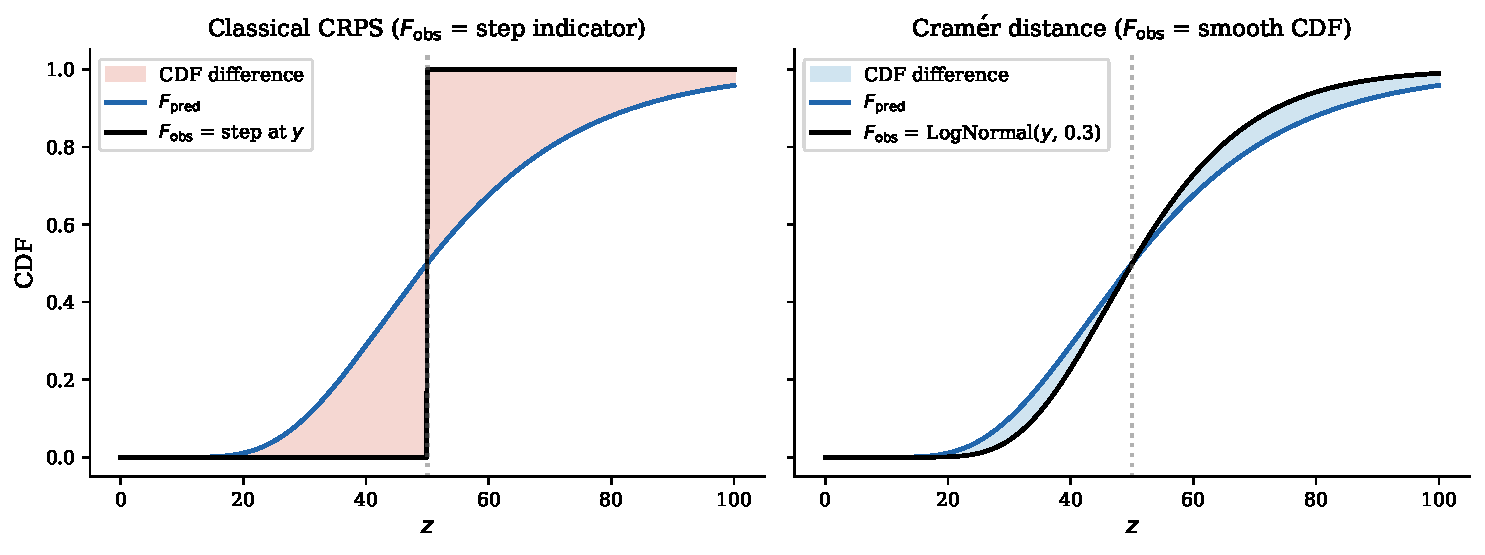
\includegraphics[width=\textwidth]{figures/step_vs_sigmoid.pdf}
    \caption{CDF comparison under two definitions of $F_\text{obs}$. Left: classical CRPS uses a step indicator; the shaded area between the smooth forecast and the hard boundary is large. Right: the Cram\'er-distance reformulation uses a smooth $F_\text{obs}$ reflecting observational uncertainty; a moderately wide forecast is no longer penalised relative to an overconfident one. The shaded region shows the gap $F_\text{pred}(z) - F_\text{obs}(z)$; the Cram\'er-distance integrand is its square.}
    \label{fig:step_vs_sigmoid}
\end{figure}


\section{The Cram\'er-Distance Reformulation}
\paragraph{Reformulation.}
The fix is straightforward: instead of comparing the forecast against a hard step at the reported value, I compare it against a smooth distribution that represents what is actually known about the observation. Concretely, I replace the step indicator in the CRPS integrand with a smooth observational CDF $F_\text{obs}(z)$:
%
\begin{equation}
    \text{CRPS}_\text{obs}(F_\text{pred}, F_\text{obs}) = \int_{-\infty}^{\infty} \bigl( F_\text{pred}(z) - F_\text{obs}(z) \bigr)^2 \, dz.
    \label{eq:fuzzy_crps}
\end{equation}
%
When $F_\text{obs}$ degenerates to a step function at the reported value $y$, the integral reduces exactly to classical CRPS. When $F_\text{obs}$ has positive variance, the integrand is smaller for forecasts that match $F_\text{obs}$ and larger for forecasts that deviate in either direction.

\paragraph{Identification with the Cram\'er distance.}
The integral in Eq.~\ref{eq:fuzzy_crps} is a known mathematical object---the Cram\'er distance between $F_\text{pred}$ and $F_\text{obs}$, measuring the total squared area between two probability curves \citep{cramer1946}.\footnote{The Cram\'er distance is closely related to the energy distance of \citet{szekely2013energy}: $\int(F - G)^2\,dz = \tfrac{1}{2}\,\varepsilon(F,G)$ in the univariate case.} In forecast verification, \citet{thorarinsdottir2013using} define the same integral as the \emph{Integrated Quadratic Distance} (IQD) and apply it to evaluate climate model output against reanalysis distributions---both non-degenerate CDFs. Classical CRPS is the special case where $F_\text{obs}$ degenerates to a step function at a single point; Eq.~\ref{eq:fuzzy_crps} is the general form applied to a non-degenerate $F_\text{obs}$. (Some authors reserve ``Cram\'er distance'' for the square root of this integral, following the convention that a distance inherits the $L^2$ norm; I use it throughout for the integral itself, following \citealt{thorarinsdottir2013using}.)

\paragraph{Constructing $F_\text{obs}$.}
The proposal is only as useful as the choice of $F_\text{obs}$. I provide three constructors---principled demonstrations of how to build $F_\text{obs}$ from available data---ordered from most data-rich to most generic.

\subsection*{Constructor 1: Dataset quality bounds}
Many event datasets provide explicit low/best/high estimates per observation. The UCDP Georeferenced Event Dataset \citep{ucdp_codebook}, for instance, records best, low, and high fatality estimates derived from the coding process---these bounds represent coder disagreement about the plausible range, not quantiles of a measurement-error distribution. I treat them pragmatically as the support of either a uniform or a log-normal distribution centred on the best estimate:
%
\begin{equation}
    F_\text{obs}(z) = \text{Uniform}(z; \text{low}, \text{high})
    \quad \text{or} \quad
    F_\text{obs}(z) = \text{LogNormal}(z; \log(\text{best}), \sigma_\text{LN})
\end{equation}
%
where $\sigma_\text{LN}$ is set so that approximately 95\% of mass falls in $[\text{low}, \text{high}]$. This is the most principled constructor because it uses the dataset's own quality metadata, external to the forecaster being evaluated.

\subsection*{Constructor 2: RVI Gumbel mixture}
\citet{vesco2026uncertainty} asked conflict-data coders to estimate plausible ranges for a set of reported fatality counts. The responses revealed a consistent pattern: some fraction of coders effectively reproduced the reported value, while the remainder believed the true count was likely higher. Vesco et al.\ capture this in a Reported-Value Inflated (RVI) Gumbel mixture model, where the Gumbel component is a right-skewed distribution that places more probability mass above the reported value than below---matching the asymmetric direction of conflict-fatality underreporting. The RVI CDF is
%
\begin{equation}
    F_\text{obs}(z) = w \cdot \mathbf{1}(z \geq \tilde{y}) + (1 - w) \cdot \text{Gumbel}(z; \mu_\text{g}, \beta_\text{g}),
\end{equation}
%
where $w$ is the probability mass on the reported value $\tilde{y}$, and $(\mu_\text{g}, \beta_\text{g})$ are the Gumbel location and scale. The location and scale parameters $(\mu_\text{g}, \beta_\text{g})$ are predicted from $\log(1 + \tilde{y})$ and vague-number indicator dummies via linear regression; $w$ is predicted from the same covariates via logistic regression. I use the coefficient estimates from Table~A10 in \citet{vesco2026uncertainty}, which pools across violence types (36 coefficients total: intercept + slope for each of $w$, $\mu_\text{g}$, $\beta_\text{g}$, plus vague-number terms).\footnote{The implementation clamps $w \in [0.01, 0.99]$ and $\mu_g \geq 0$ to prevent degenerate predictions; the Gumbel CDF assigns non-zero probability to negative fatalities, which is handled by truncating at zero.} This constructor captures the asymmetric underreporting that symmetric parametric constructors miss: for low-fatality events, where underreporting is most severe, the Gumbel tail spreads substantially above the reported count. The vague-number indicator dummies are designed for event-level reported values; applying them to cell-month aggregates is a known approximation (see \S7 for discussion). Where UCDP data are available, this constructor supersedes the parametric default.

\subsection*{Constructor 3: Parametric default}
For datasets without explicit bounds or an empirical uncertainty model, a default is a log-normal centred on the reported value with a fixed relative uncertainty:
%
\begin{equation}
    F_\text{obs}(z) = \text{LogNormal}\bigl(z; \log(y), \sigma_\text{rel}\bigr).
\end{equation}
%
The parameter $\sigma_\text{rel}$ should be informed by domain knowledge---the typical revision rate between successive dataset releases, the known underreporting ratio, or expert elicitation. For armed-conflict fatality counts, I use $\sigma_\text{rel} = 0.4$ as a working default. In practice, this places roughly two-thirds of the observational distribution between $0.67y$ and $1.49y$---for a reported count of 50 deaths, the plausible range runs from about 34 to 75. The RVI Gumbel model of \citet{vesco2026uncertainty} (Constructor~2) implies that the effective log-space standard deviation of observational uncertainty varies from approximately 0.2 for large events ($\tilde{y} > 100$) to over 0.9 for single-fatality events; $\sigma_\text{rel} = 0.4$ approximates the range typical of small-to-medium events. Where event-specific uncertainty is available, Constructor~2 supersedes this parametric default. A community using this reformulation for benchmarking would need to agree on standard $\sigma_\text{rel}$ values per data type, analogous to standardised baselines in forecast competitions.

\paragraph{Numerical implementation.}
The integral in Eq.~\ref{eq:fuzzy_crps} is computed by trapezoidal integration over a uniform grid of 4{,}001 points covering the support of both $F_\text{pred}$ and $F_\text{obs}$. Forecast CDFs are represented as empirical CDFs from 4{,}000 Monte Carlo samples (random draws used to approximate the CDF numerically; seed~$= 0$ throughout). Doubling the grid to 8{,}001 points changes scores by $< 0.01\%$; doubling the Monte Carlo sample to 8{,}000 changes individual scores by up to ${\sim}4\%$ but does not affect rankings. For specific parametric families where both CDFs are log-normal, closed-form expressions for the IQD exist; the reference implementation uses the general numerical form to accommodate arbitrary $F_\text{obs}$ constructors.


\section{Consistency Properties}
The Cram\'er distance between two fixed CDFs is a proper divergence: it is non-negative and equals zero if and only if the two distributions are identical \citep{szekely2013energy,thorarinsdottir2013using}. This is a weaker guarantee than the classical propriety of \S2---it says that the best forecast \emph{for a given observation} is the observation itself, but does not directly address what happens when the observation is stochastic.

The substantive question is whether the pipeline---constructing $F_\text{obs}$ from a noisy draw $y$ and scoring $F_\text{pred}$ against it---rewards forecasts that get the location right. I verify this numerically: drawing $N = 500$ observations from a known distribution, constructing $F_\text{obs}$ for each draw, and sweeping a forecast parameter $\mu$ across a grid. The argmin falls at the true $\mu$ to within grid resolution for all tested values across three distributional families (log-normal, Gaussian, count-like); a refined sweep at $\Delta\mu = 0.005$ with $N = 2{,}000$ draws confirms residual bias $\leq 0.01$ (Appendix~\ref{sec:appendix_consistency}). One limiting case is analytically tractable: as $\sigma_\text{rel} \to 0$, each $F_\text{obs}(y)$ converges pointwise to the step function at $y$, so the Cram\'er distance reduces to classical CRPS by dominated convergence, and location-consistency follows from strict propriety \citep{gneiting2007strictly}. Underestimation of observational uncertainty therefore degrades gracefully to the classical regime. A formal proof of location-consistency for the general case via the energy-distance framework is beyond the scope of this paper.

Scale-consistency does \emph{not} hold: the minimising spread absorbs the observation noise, just as a blurred photograph combines camera-shake and lens-blur into a single effective width. For conflict fatality data, this effect is more consequential than in meteorology or hydrology: the RVI model of \citet{vesco2026uncertainty} implies observational uncertainty of $\sigma_\text{rel} \approx 0.2$--$0.7$ in log-space, which can equal or exceed forecast-model spread. The metric rewards forecasts that match the observable data distribution, not the latent truth---the same property classical CRPS has in degenerate form. This does not affect the ranking reversals demonstrated in \S6, which depend on location-consistency rather than scale-consistency. Formal details---including the $L^2$ minimisation proof, the stochastic-observation consistency definition, numerical verification, and the full scale-consistency analysis---are in Appendix~\ref{sec:appendix_consistency}.


\section{Demonstration}
\subsection{Controlled demonstration}

\paragraph{Setup.}
Does accounting for observational uncertainty change which forecast version wins? I start with a controlled case: both versions are centred on the reported value $y$, which isolates the spread dimension---both metrics handle location identically. The setup:

\begin{itemize}
    \item The reported observation is $y = 50$.
    \item The assumed observational uncertainty is $\sigma_\text{rel} = 0.4$ in log-space (the Constructor~3 working default; see \S3 for calibration against the RVI Gumbel model).
    \item Two forecast versions predict the same observation:
    \begin{itemize}
        \item \textbf{Tight (overconfident):} LogNormal($\log y$, $\sigma_\text{tight} = 0.05$)---concentrates nearly all probability mass on a single value, claiming to know the truth precisely.
        \item \textbf{Honest:} LogNormal($\log y$, $\sigma_\text{honest} = 0.4$)---a wider distribution matching the true observational uncertainty.
    \end{itemize}
\end{itemize}

\paragraph{Results.}
Classical CRPS ranks the tight version first: its narrow distribution is closer to the step at $y$ at almost every $z$, and the squared-area integrand is smaller. The reformulated metric, computed against a smooth $F_\text{obs}$ constructed via Constructor~3 ($\sigma_\text{rel} = 0.4$), reverses the ranking: the honest version wins. Figure~\ref{fig:reversal} shows the four scores. The reversal is qualitative, not a numerical artifact. In this baseline case, the reversal is algebraically guaranteed: the Cram\'er distance is an $L^2$ metric, and $\sigma_\text{honest} = \sigma_\text{rel}$ means the honest version's CDF matches $F_\text{obs}$ exactly, which is the minimiser by construction. The substantive question is not \emph{whether} the reversal occurs at the matched parameterisation, but \emph{how far} the honest version can deviate from $F_\text{obs}$ and still beat the overconfident version.

\begin{figure}[h]
    \centering
    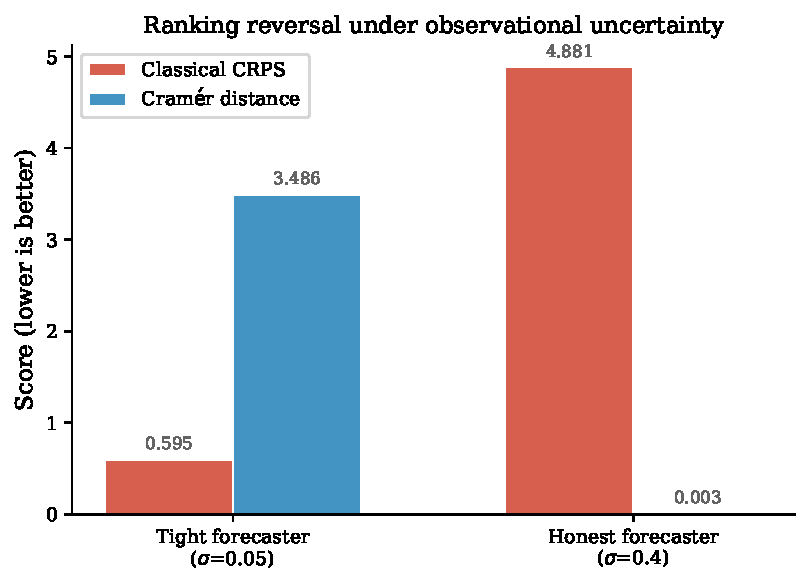
\includegraphics[width=0.7\textwidth]{figures/uncertainty_aware_ranking.pdf}
    \caption{Ranking reversal between two forecast versions on a controlled example. Under classical CRPS the tight (overconfident) version wins; under the Cram\'er-distance reformulation the honest version wins. The reversal is qualitative---the sign of which version is better changes.}
    \label{fig:reversal}
\end{figure}

The reversal does not depend on the honest version exactly matching $F_\text{obs}$: varying $\sigma_\text{honest}$ while holding $\sigma_\text{rel} = 0.4$ fixed, the reversal holds for $\sigma_\text{honest} \in [0.10, \, 0.85]$---the honest version can be $4\times$ too narrow or $2\times$ too wide and still beat the tight version. The reversal disappears when observational uncertainty is small ($\sigma_\text{rel} \leq 0.10$) or when the honest version is extremely wide ($\sigma_\text{honest} \geq 1.0$). Detailed robustness analysis---including constructor comparison, location-error tolerance, and generalisation across distributional families---is in Appendix~\ref{sec:appendix_demo}.

\subsection{Empirical comparison on UCDP conflict data}

\paragraph{Data and design.}
I replicate the controlled demonstration on real observations from the UCDP Georeferenced Event Dataset (GED, data version 24.1, final-coded events; codebook: \citealt{ucdp_codebook}), using best-estimate fatality counts from 2020--2024 aggregated to the PRIO-GRID cell-month level (a $0.5^\circ \times 0.5^\circ$ geographic grid cell observed in a single calendar month, the standard spatiotemporal unit in VIEWS-format evaluations). I pool state-based, non-state, and one-sided violence and retain cell-months with at least one recorded fatality; historical uncertainty is derived from cells with $\geq 3$ active months during 1989--2019. This yields 19{,}397 cell-months from 2{,}065 cells. This sample covers the active-conflict portion of the evaluation space; the roughly 800{,}000 cell-months with zero recorded fatalities are excluded because $F_\text{obs}$ degenerates to a step function at zero and the reformulation reduces to classical CRPS. The results therefore characterise the regime where observational uncertainty is operative, not the full VIEWS evaluation grid.

For each cell-month I construct two forecast versions, both centred on the reported best estimate $y$:
\begin{itemize}
    \item \textbf{Tight:} $\text{LogNormal}(\log y, \, 0.05)$---claims to know the observation precisely.
    \item \textbf{Honest:} $\text{LogNormal}(\log y, \, \hat{\sigma}_\text{cell})$---where $\hat{\sigma}_\text{cell} = \sqrt{\log(1 + \text{CV}^2)}$ is derived from the cell's historical coefficient of variation. Median $\hat{\sigma}_\text{cell} = 0.97$; interquartile range $[0.81, 1.16]$; clipped to $[0.1, 2.0]$ (affecting 1.1\% of cell-months).
\end{itemize}
I score both under classical CRPS and the Cram\'er-distance reformulation with Constructor~3 ($\sigma_\text{rel} = 0.4$).

\paragraph{Results.}
Under classical CRPS the tight version wins in 100\% of cell-months---a direct consequence of both versions being centred on $y$ and CRPS's well-known preference for concentration. Under the Cram\'er-distance reformulation, the ranking reverses in 39\% of cell-months overall.\footnote{The reversal rate is sensitive to $\sigma_\text{rel}$: at $\sigma_\text{rel} = 0.3$ it drops to 12.6\%; at $\sigma_\text{rel} = 0.5$ it rises to 67.7\%.} The reversal rate depends sharply on forecast uncertainty: for cells with moderate uncertainty ($\hat{\sigma}_\text{cell} \leq 0.8$; $n = 4{,}716$), the honest version wins in \emph{every} cell-month. For cells with very high uncertainty ($\hat{\sigma}_\text{cell} > 1.0$; $n = 8{,}902$), the honest version is too wide and loses---exactly the regime identified in the controlled demonstration. Figure~\ref{fig:real_data} shows the reversal rate by uncertainty regime and the score-difference distribution.

\begin{figure}[h]
    \centering
    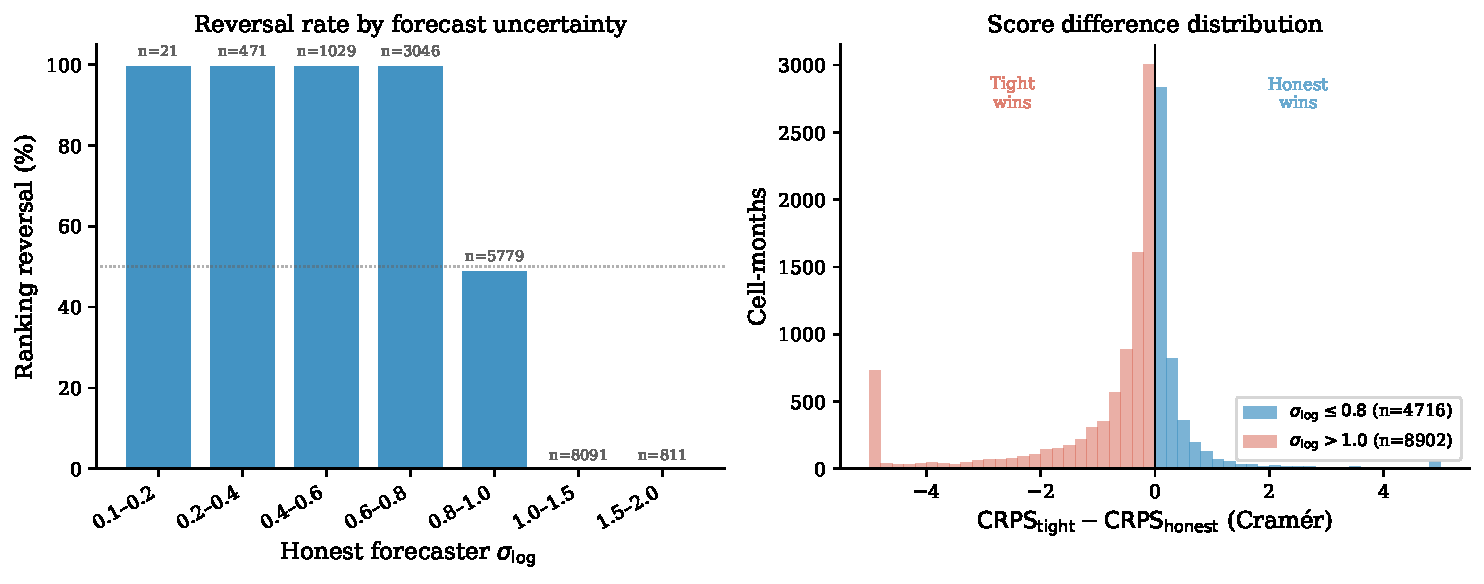
\includegraphics[width=\textwidth]{figures/real_data_comparison.pdf}
    \caption{Ranking reversal on UCDP conflict data (2020--2024, 19{,}397 cell-months). Left: reversal rate under the Cram\'er-distance reformulation as a function of the honest version's log-space uncertainty $\hat{\sigma}_\text{cell}$. The reversal is complete for $\hat{\sigma}_\text{cell} \leq 0.8$ and absent for $\hat{\sigma}_\text{cell} > 1.0$. Right: distribution of score differences; positive values indicate the honest version wins.}
    \label{fig:real_data}
\end{figure}

Among cell-months with genuine UCDP low/best/high bounds, Constructor~1 produces a reversal rate of only 9.9\%---reflecting the fact that UCDP's coding ranges are narrow relative to the true observational uncertainty \citep{vesco2026uncertainty}. Under the RVI Gumbel mixture (Constructor~2), the reversal widens to 80.8\% of cell-months, capturing asymmetric underreporting that the symmetric parametric constructor misses. The Bessac--Naveau conditional-expectation correction \citep{bessac2021forecast} confirms the pattern, with 98.1\% concordance overall. A per-violence-type breakdown, constructor comparison details, and the unit-of-analysis caveat for Constructor~2 are in Appendix~\ref{sec:appendix_demo}.

\subsection{Validation with an operational forecaster}

The preceding comparisons centre both versions on the reported value $y$---information unavailable at prediction time. This isolates the spread effect but leaves open whether the reversal survives when the model does not observe $y$. I test this using HydraNet \citep{VonDerMaase2025hydranet}, a spatio-temporal Monte Carlo Dropout architecture trained on the Violence \& Impacts Early-Warning System (VIEWS) PRIO-GRID. The model produces 64 posterior samples per cell-month\footnote{The HydraNet architecture draws 128 samples per cell-month in its reference configuration; the validation here uses 64 due to local memory constraints.} for each violence type; I use state-based fatalities, the best-documented violence type with the lowest reversal rate in the synthetic comparison (79.3\% under RVI; Appendix~\ref{sec:appendix_demo})---the reformulation's impact is likely larger for non-state and one-sided violence, where observational uncertainty is greater.

\paragraph{Setup.}
The model is trained on January 1990--December 2020 and produces 36-step-ahead validation predictions for January 2021--December 2024 (the standard VIEWS validation partition). I match these against UCDP state-based fatality actuals aggregated to the cell-month level, using the shortest-horizon (most recent) prediction available for each cell-month, yielding 6{,}725 cell-months across 1{,}173 cells where the reported best estimate is positive. For each cell-month, I construct two versions of the same model's output---this tests whether the metric values uncertainty quantification, not whether it changes model selection between genuinely different systems:
\begin{itemize}
    \item \textbf{Full posterior:} the model's 64 posterior samples, used directly as the forecast distribution.
    \item \textbf{Tight:} $\text{LogNormal}(\log \bar{x}, \, 0.05)$ where $\bar{x}$ is the posterior mean---a version that retains the model's location estimate but discards its uncertainty quantification.
\end{itemize}
Both versions share the same location; the only difference is spread.

\paragraph{Results.}
In the full sample, classical CRPS strictly prefers the tight version in only 2.5\% of cell-months (167/6{,}725). A further 16.4\% (1{,}102 cell-months) are ties where the model predicts zero fatalities and both versions are degenerate; the remaining 81.1\% strictly prefer the full posterior. The dominance of the full posterior reflects HydraNet's typically large location errors; when the model misses the location, wider spread helps under classical CRPS simply by placing more mass near the target.

The interesting regime is the 1{,}031 cell-months (15.3\%) where the model's prediction falls within a factor of two of the actual---where location error is moderate and the spread dimension becomes consequential. In this subset, classical CRPS selects the tight version in 167 cell-months (16.2\%). The Cram\'er-distance reformulation (Constructor~3, $\sigma_\text{rel} = 0.4$) reverses 166 of these 167 cases (99.4\%), selecting the full posterior instead. Under the RVI Gumbel constructor (Constructor~2), the reversal rate is 167/167 (100\%). The single cell-month that resists reversal under Constructor~3 is a high-fatality case (best $= 56$) where the full posterior has a log-space standard deviation of $0.77$---genuinely too wide relative to $F_\text{obs}$. The Cram\'er distance does not reward uncertainty indiscriminately but penalises spread that exceeds observational uncertainty, exactly as in the synthetic demonstration.


\section{Discussion}
\paragraph{Choosing $F_\text{obs}$ in practice.}
The three constructors have different epistemic credentials. Dataset quality bounds (Constructor~1) are the most defensible because they are external to the forecaster being evaluated; the low 9.9\% reversal rate under Constructor~1 (\S5) itself suggests that UCDP coding ranges understate true observational uncertainty. Parametric defaults (Constructor~3) are practical but introduce a free parameter; a careless choice of $\sigma_\text{rel}$ can mask or invert the ranking, and benchmarking communities would need to agree on standard values per data type. The RVI Gumbel mixture (Constructor~2) bridges these approaches: it uses regression coefficients estimated from coder surveys \citep{vesco2026uncertainty} to predict the distribution of plausible fatality counts, capturing the asymmetric underreporting that symmetric parametric constructors miss. The Vesco et al.\ model has its own limitations---response biases in coder surveys, assumed distributional form, limited sample size---and should be read as a principled estimate rather than ground truth. That said, I recommend Constructor~2 where UCDP data are available, Constructor~1 where quality bounds exist for other datasets, and Constructor~3 with a community-agreed $\sigma_\text{rel}$ otherwise. A caveat: the Constructor~2 results in \S5 apply the RVI regression at the cell-month aggregate level rather than per event, introducing a unit-of-analysis mismatch that likely understates the true observational uncertainty (see \S5); event-level application would be more principled but requires combining event-level distributions. A fourth possibility---deriving $F_\text{obs}$ from a model's own confidence signal---is conceptually available but introduces circularity; I do not pursue it here.

\paragraph{Relation to prior approaches.}
The problem of evaluating forecasts against imprecise observations is well studied; the present work applies ideas developed primarily in meteorology to conflict forecasting. One structural consequence worth noting first: \citet{brocker2009reliability} decomposes proper scores into reliability, resolution, and uncertainty components; the Cram\'er-distance reformulation shifts mass from the ``uncertainty'' term---which in the classical decomposition absorbs all observational noise---into the smooth $F_\text{obs}$ in the integrand. A formal restatement of this decomposition for the reformulated metric is deferred to a technical companion.

\textbf{Scoring under observation error.} \citet{brocker2007scoring} highlight the need for generalised scores when verification data are uncertain, proposing a convolution approach: the forecast is convolved with the observation-error kernel before scoring, so that forecast and observation are compared on equal footing. \citet{bessac2021forecast} take a different route, computing $\mathbb{E}[S(F, Y) \,|\, \tilde{y}]$---the conditional expectation of the score over the observation error distribution---yielding an unbiased estimate of the true score. This conditional-expectation correction is principled when the observation error model is known. The Cram\'er-distance reformulation takes a third route: rather than correcting the score after the fact, it replaces the degenerate observation CDF with a smooth $F_\text{obs}$ \emph{inside the integrand}, changing what is being measured. The Br\"ocker--Smith convolution asks ``what would the score look like if the forecast absorbed the observation noise?''; the Bessac--Naveau correction asks ``what would the score have been had we observed the truth?''; the Cram\'er-distance reformulation asks ``what is the distance between the forecast distribution and the observation distribution?'' The three approaches yield the same ranking in expectation when $F_\text{obs}$ is correctly specified, but they differ in what they require: the convolution approach requires a noise kernel, the conditional-expectation approach requires a tractable posterior $[X \mid Y]$, and the CDF-substitution approach requires a constructable $F_\text{obs}$.

I verify this empirically by comparing the Cram\'er-distance reformulation against the Bessac--Naveau conditional-expectation correction. On the controlled demonstration (\S5), both approaches select the same winner (honest version) for all $\sigma_\text{honest} \leq 0.80$ and agree that the tight version wins for $\sigma_\text{honest} \geq 0.90$. A narrow disagreement band exists at $\sigma_\text{honest} \approx 0.85$--$0.88$, where the Cram\'er distance still selects the honest version but the conditional-expectation correction flips to tight---the CDF-substitution approach is slightly more tolerant of wide versions near the transition. On the UCDP empirical comparison (19{,}397 cell-months, Constructor~3 with $\sigma_\text{rel} = 0.4$), the two approaches agree in 98.1\% of cell-months overall. Outside the transition zone ($\hat{\sigma}_\text{cell} \leq 0.8$ or $> 1.0$) concordance is 100\%; within the transition zone ($0.8 < \hat{\sigma}_\text{cell} \leq 1.0$) it drops to 93.6\%---roughly one in fifteen cell-months receives a different ranking depending on the method (\S5). The residual disagreement is concentrated precisely where the decision is hardest: where observational uncertainty is large enough to be consequential but not so large as to swamp the forecast signal. In this disagreement band, the conditional-expectation correction has the stronger theoretical warrant---it recovers an unbiased estimate of the true score under correct error-model specification---whereas the Cram\'er distance measures a different quantity (distribution-to-distribution distance) whose optimality depends on the $F_\text{obs}$ constructor.

\textbf{Error-corrected and distributional approaches.} \citet{ferro2017observation} constructs error-corrected proper scoring rules whose expected values, taken over the observation-error distribution, equal the original proper score evaluated at the true value---a frequentist unbiasedness condition that requires an explicit error model but not a Bayesian posterior. \citet{candille2008impact} study the impact of observation error on ensemble verification diagnostics, proposing an ``observational-probability'' method that replaces point observations with probability distributions in scores such as the Brier score and reliability diagrams. \citet{bessac2021forecast} derive the full distribution of CRPS under Gaussian additive and multiplicative-Gamma observation errors, showing that imperfect verification data cause systematic underdispersion bias---an effect closely related to the ranking reversal demonstrated in \S5.

The underdispersion bias Bessac and Naveau predict analytically is directly observable in the UCDP data (\S5): classical CRPS selects the tight version in 100\% of cell-months, and the Cram\'er-distance reformulation reverses this in precisely the regime where observational uncertainty exceeds forecast uncertainty (Spearman $\rho = -0.38$, $p < 10^{-15}$, between $\sigma_\text{honest}$ and the classical score gap).

These approaches share the same motivation as the present work but address different aspects: score bias (Bessac--Naveau), error-corrected scoring (Ferro), or diagnostic calibration (Candille--Talagrand), whereas I focus on the effect on model ranking.

\textbf{Scale-sensitivity and ensemble size.} \citet{bolin2023local} show that CRPS is not locally scale-invariant: it overweights observations in regions where the forecast distribution has large variability. They propose a Scaled CRPS that normalises by local spread---a complementary approach that could in principle be combined with the reformulation proposed here. \citet{ferro2017fair} addresses finite ensemble size bias, a distinct but related source of overconfidence in CRPS rankings. \citet{weijs2011accounting} cast the problem in information-theoretic terms, proposing divergence-based scores with explicit uncertainty decompositions; their framework is more general but requires different scoring infrastructure.

Among these approaches, the Cram\'er-distance reformulation is attractive for domains where observation error models are not well characterised: it requires only a constructable $F_\text{obs}$, not an invertible error model, and reduces exactly to classical CRPS when observations are precise. Its main advantage for conflict forecasting is that it provides a natural entry point for empirically grounded uncertainty models: UCDP's own low/best/high bounds are coding artefacts that understate the true observational uncertainty (\S5), but the RVI Gumbel mixture of \citet{vesco2026uncertainty}---built precisely because those bounds are insufficient---can be plugged directly into the $F_\text{obs}$ constructor. Fields with well-characterised instrument error covariances (e.g.\ numerical weather prediction) may benefit more from the conditional-expectation correction of \citet{bessac2021forecast}, the convolution approach of \citet{brocker2007scoring}, or the error-corrected scoring rules of \citet{ferro2017observation}.

\paragraph{What the reformulation does not solve.}
\begin{itemize}
    \item \textbf{It does not solve the Forecaster's Dilemma.} The result of \citet{lerch2017forecasters}---that conditioning forecast evaluation on extreme observations systematically discredits skillful forecasts---holds for the reformulated metric just as for classical CRPS. Weighted scoring rules that emphasise tail behaviour \citep{gneiting2011comparing} are still needed as complementary diagnostics.

    \item \textbf{It does not eliminate distributional assumptions.} The constructor of $F_\text{obs}$ is itself a distributional assumption. The reformulation moves the assumption from ``observations are exact'' to ``observations follow this distribution''---more honest, but still an assumption open to mis-specification.

    \item \textbf{Additional sources of observational uncertainty are unaddressed.} Systematic data-quality biases, spatial variation in reporting quality, georeferencing imprecision (UCDP precision codes 1--7), and false-negative uncertainty in the roughly 800{,}000 zero-fatality cell-months excluded from \S5 each represent distinct error sources not captured by $F_\text{obs}$.

    \item \textbf{The demonstrations use oracle-centred forecast versions.} The controlled and UCDP comparisons centre both versions on the reported value $y$---information unavailable at prediction time. The 39\% reversal rate describes a regime of perfect location knowledge; the HydraNet validation (\S5.3) tests whether the reversal survives genuine location error. All three comparisons test uncertainty valuation rather than model selection---whether the reformulation changes rankings between genuinely different models is untested.
\end{itemize}

\paragraph{Sensitivity to $F_\text{obs}$ mis-specification.}
Could the metric's behaviour under a mis-specified $F_\text{obs}$ be worse than classical CRPS with no $F_\text{obs}$ at all? I quantify this by running the stochastic consistency check from \S4 (details in Appendix~\ref{sec:appendix_consistency}) under deliberate mis-specification. The true data-generating distribution is $\text{LogNormal}(\mu = 1.0, \sigma = 0.3)$; I construct $F_\text{obs}$ using $\sigma_\text{rel}$ values ranging from $0.1$ to $1.0$ and ask where the expected Cram\'er distance is minimised.

Table~\ref{tab:misspec} shows the results. When $\sigma_\text{rel}$ matches the true $\sigma$ (ratio 1.0$\times$), the argmin falls exactly on $\mu_\text{true}$. Moderate overestimation (up to 2$\times$) shifts the argmin by at most one grid step ($+0.05$). Severe overestimation (3.3$\times$) shifts it by $+0.15$---meaningful but bounded. Underestimation produces no detectable bias in this sweep. For this log-normal DGP, the bias is monotonic in the mis-specification ratio; whether monotonicity holds across distributional families is untested, but the practical implication---a practitioner can bound the bias by bounding the mis-specification---applies whenever the relationship is monotone.

The asymmetry has a structural explanation. When $\sigma_\text{rel}$ is underestimated, $F_\text{obs}$ approaches the degenerate step function at $y$, and the Cram\'er distance reduces to classical CRPS---which is proper, so the location argmin remains at $\mu_\text{true}$. When $\sigma_\text{rel}$ is overestimated, $F_\text{obs}$ is wider than the true observation noise; the log-normal right-skew of the widened $F_\text{obs}$ shifts the $L^2$-minimising location upward, producing positive bias. The same mechanism explains the scale-consistency convolution effect discussed in \S4 and Appendix~\ref{sec:appendix_consistency}: the metric measures distance from the observable distribution, which inherits the observation noise.

A formal characterisation of this bias is an open problem.

\begin{table}[h]
    \centering
    \small
    \begin{tabular}{rrrr}
        \toprule
        $\sigma_\text{rel}$ & Ratio ($\sigma_\text{rel} / \sigma_\text{true}$) & Argmin $\hat{\mu}$ & Bias ($\hat{\mu} - \mu_\text{true}$) \\
        \midrule
        0.1 & 0.3$\times$ & 1.000 & 0.000 \\
        0.2 & 0.7$\times$ & 1.000 & 0.000 \\
        0.3 & 1.0$\times$ & 1.000 & 0.000 \\
        0.4 & 1.3$\times$ & 1.050 & $+$0.050 \\
        0.6 & 2.0$\times$ & 1.050 & $+$0.050 \\
        0.8 & 2.7$\times$ & 1.100 & $+$0.100 \\
        1.0 & 3.3$\times$ & 1.150 & $+$0.150 \\
        \bottomrule
    \end{tabular}
    \caption{Argmin bias under mis-specified $F_\text{obs}$. The true DGP is $\text{LogNormal}(1.0, 0.3)$; $F_\text{obs}$ uses varying $\sigma_\text{rel}$. Monte Carlo expectation over 500 draws. Grid step $= 0.05$.}
    \label{tab:misspec}
\end{table}

\paragraph{Implications for forecast competitions.}
Forecast competitions and model selection procedures that use CRPS as the sole ranking metric implicitly assume observations are exact. When this assumption is violated, competition rankings can systematically favour overconfident models. The practical recommendation is not to replace CRPS with the Cram\'er-distance reformulation in all settings---classical CRPS is exactly right when observations are precise---but to use the reformulation as a secondary metric or robustness check in domains where observational uncertainty is known to be substantial. This recommendation rests on location-consistency verified numerically across three distributional families (\S5; Appendix~\ref{sec:appendix_demo}, Table~\ref{tab:multi_dgp}). Domains where this is immediately relevant include conflict forecasting \citep{hegre2019views,ucdp_codebook}, epidemiological surveillance \citep{gibbons2014measuring}, and economic forecasting from survey data.

\paragraph{Open questions.}
\begin{itemize}
    \item Closed-form expressions for the reformulated metric when both $F_\text{pred}$ and $F_\text{obs}$ belong to common parametric families (log-normal, gamma, Weibull) would speed evaluation and enable analytical optimisation.
    \item A formal Br\"ocker decomposition of the reformulated metric into reliability, resolution, and observational-uncertainty components.
    \item An analytical proof of consistency under stochastic observations via the energy-distance framework, with explicit conditions on the $F_\text{obs}$ constructor.
    \item Empirical comparison of model rankings on operational benchmarks (conflict forecasting, weather prediction, epidemiological surveillance) under classical and reformulated CRPS with each constructor.
    \item Convergence analysis: how does the bias from a mis-specified $F_\text{obs}$ scale with the magnitude and direction of the mis-specification?
\end{itemize}


\appendix

\section{Consistency Properties: Formal Details}
\label{sec:appendix_consistency}
\paragraph{$L^2$ minimisation (fixed $F_\text{obs}$).}
For any fixed observational CDF $F_\text{obs}$, the integral
$\int (F_\text{pred}(z) - F_\text{obs}(z))^2\,dz$
is non-negative and equals zero if and only if $F_\text{pred}(z) = F_\text{obs}(z)$ for all $z$. The minimiser over deterministic $F_\text{pred}$ is therefore $F_\text{obs}$ itself. This is an $L^2$ minimisation statement, not a propriety theorem in the \citet{gneiting2007strictly} sense---classical propriety requires an expectation over the random observation $y$, which the fixed-$F_\text{obs}$ statement does not involve.

\paragraph{Consistency under stochastic observations.}
Write $F_\text{obs}(y)$ for the observational CDF built from a specific draw $y$. The relevant quantity is
%
\begin{equation}
    \mathbb{E}_{y \sim Q} \bigl[ \text{CRPS}_\text{obs}(F_\text{pred}, F_\text{obs}(y)) \bigr].
\end{equation}
%
The metric should reward forecasts that get the location right, even when individual observations are noisy. Formally, I say that the pipeline is \emph{location-consistent} at $F_\text{pred} = Q$ if this expectation is minimised over the forecast location parameter when $F_\text{pred}$ equals the true data-generating distribution $Q$. Consistency in this sense is weaker than classical propriety---it depends on the $F_\text{obs}$ constructor being well-specified with respect to $Q$---but it is the property a practitioner needs: reporting the true location should yield the best expected score.

The honesty of the metric depends on the honesty of the $F_\text{obs}$ constructor. A practitioner who specifies $\sigma_\text{rel} = 0.3$ when the true relative uncertainty is 0.1 will get a metric that rewards forecasts that are too wide; one who specifies $\sigma_\text{rel}$ too small will get a metric that rewards overconfidence. The reformulation does not eliminate the distributional assumption---it moves it from inside the score formula to the constructor of $F_\text{obs}$, where it is visible, auditable, and open to sensitivity analysis.

\paragraph{Numerical consistency check.}
I verify consistency by drawing $N = 500$ observations $y^{(1)}, \ldots, y^{(N)}$ from a known log-normal truth with parameters $\mu_\text{true}$ and $\sigma = 0.3$ (a test parameter chosen for the numerical check; the operational default for conflict data is $\sigma_\text{rel} = 0.4$, \S3), constructing $F_\text{obs}(y^{(i)})$ parametrically for each draw with $\sigma_\text{rel} = 0.3$, sweeping a forecast parameter $\mu$ across a grid, and computing the expected score $\frac{1}{N}\sum_i \text{CRPS}_\text{obs}(F_\text{pred}(\mu), F_\text{obs}(y^{(i)}))$ for each $\mu$. The argmin should fall near $\mu_\text{true}$.

Figure~\ref{fig:propriety} shows the result for $\mu_\text{true} = 1.0$. At grid step $\Delta\mu = 0.05$ ($N = 500$ draws), the argmin falls on $\mu = 1.0$ for all four tested values $\mu_\text{true} \in \{0.5, 1.0, 1.5, 2.0\}$. Refining to $\Delta\mu = 0.005$ with $N = 2{,}000$ draws, the residual bias is $\leq 0.01$ and varies by seed---consistent with Monte Carlo noise at the grid resolution rather than a systematic shift.

\begin{figure}[h]
    \centering
    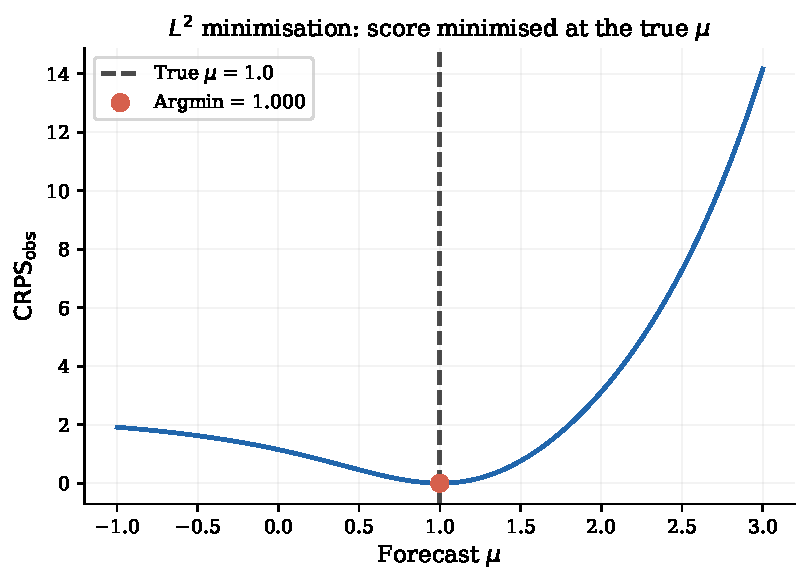
\includegraphics[width=0.65\textwidth]{figures/propriety_verification.pdf}
    \caption{Location-consistency check. The expected Cram\'er distance, averaged over $N = 500$ stochastic draws of $y$ from the true distribution (each with its own $F_\text{obs}(y^{(i)})$), is minimised at the true $\mu$.}
    \label{fig:propriety}
\end{figure}

\paragraph{Scale consistency: a convolution effect.}
The $\mu$-sweep above verifies location-consistency. A natural follow-up is whether the metric is also minimised at the true scale parameter $\sigma_\text{true}$. It is not---and the reason is intuitive: the metric rewards forecasts that match the truth \emph{as it would appear through the observation process}. Just as a blurred photograph combines camera-shake and lens-blur so that the result is wider than either source alone, the metric combines forecast spread and observation noise into a single effective width. For $\text{LogNormal}(\mu = 1.0, \sigma_\text{true} = 0.3)$ with observation-noise parameter $\sigma_\text{obs} = 0.3$ (equal to $\sigma_\text{rel}$ in the well-specified case), the expected Cram\'er distance is minimised at $\sigma_\text{pred} \approx 0.42$, not $0.30$. Under a Gaussian DGP ($\mu = 50$, $\sigma_\text{true} = 15$, $\sigma_\text{obs} = 10$), the argmin falls at $\sigma_\text{pred} \approx 18 \approx \sqrt{15^2 + 10^2}$. In both cases the minimiser is the convolution width $\sqrt{\sigma_\text{true}^2 + \sigma_\text{obs}^2}$: the expectation over stochastic $y$ effectively convolves $F_\text{pred}$ with the observation noise. For conflict fatality data, this effect is more consequential than in meteorology or hydrology: the RVI model of \citet{vesco2026uncertainty} implies observational uncertainty of $\sigma_\text{rel} \approx 0.2$--$0.9$ in log-space, which can equal or exceed forecast-model spread. When $\sigma_\text{obs} \geq \sigma_\text{true}$, the convolution width is dominated by observation noise, and the scale optimum shifts substantially from the true forecast spread.

The observable distribution is $Q * F_\varepsilon$, not the latent $Q$ itself. Classical CRPS has the same property in degenerate form: when $F_\text{obs} = \delta_y$ and $y = \theta + \varepsilon$, the CRPS-optimal forecast is $Q * F_\varepsilon$, not $Q$. Consistency therefore holds for location but not for scale: the metric rewards forecasts that match the observable data distribution, penalising overconfidence relative to what the data can actually resolve.


\section{Supplementary Demonstration Results}
\label{sec:appendix_demo}
\subsection{Constructor comparison}

The controlled demonstration in \S6.1 uses Constructor~3 (parametric). Table~\ref{tab:constructor_comparison} repeats the comparison with Constructor~1 (dataset quality bounds), using UCDP-style low/best/high bounds around the same $y=50$. With wide bounds $[25, 50, 100]$---typical of events in regions with limited media coverage---the ranking reversal holds: the honest version wins. With narrow bounds $[45, 50, 55]$---typical of well-documented events---the reversal disappears and the tight version wins, which is correct: when the observation is known precisely, a tight forecast is the right answer.

\begin{table}[h]
    \centering
    \small
    \begin{tabular}{llrrl}
        \toprule
        $F_\text{obs}$ constructor & Parameters & Tight & Honest & Winner \\
        \midrule
        Classical CRPS (step at $y$) & --- & 0.595 & 4.881 & Tight \\
        Constructor 3 (parametric) & $\sigma_\text{rel} = 0.4$ & 3.486 & 0.003 & Honest \\
        Constructor 1 (bounds) & $[25, 50, 100]$ & 6.997 & 1.361 & Honest \\
        Constructor 1 (bounds) & $[45, 50, 55]$ & 0.040 & 3.373 & Tight \\
        \bottomrule
    \end{tabular}
    \caption{Scores for the tight and honest forecast versions under classical CRPS, the parametric Cram\'er-distance reformulation (Constructor~3), and the bounds-based reformulation (Constructor~1). The ranking reversal occurs when observational uncertainty is substantial---either via a wide $\sigma_\text{rel}$ or via wide low/high bounds---and disappears when bounds are narrow. The parametric constructor uses $\sigma_\text{rel} = 0.4$ (the working default defined in \S3).}
    \label{tab:constructor_comparison}
\end{table}

\subsection{Robustness and boundary conditions}

\paragraph{Boundaries.}
The reversal does not hold universally. It disappears when $\sigma_\text{rel} \leq 0.10$ (observational uncertainty is small enough that a tight forecast is genuinely correct), when $\sigma_\text{tight} \geq \sigma_\text{rel}$ (the ``tight'' version is no longer meaningfully tight), or when $\sigma_\text{honest} \geq 1.0$ (the honest version is so wide it no longer overlaps $F_\text{obs}$). The reformulation changes the ranking only when observational uncertainty is large enough to be consequential.

A natural concern is that the reversal depends on the honest version's spread exactly matching $F_\text{obs}$. It does not. Varying $\sigma_\text{honest}$ while holding $\sigma_\text{rel} = 0.4$ fixed, the reversal holds for $\sigma_\text{honest} \in [0.10, \, 0.85]$---the honest version can be 4$\times$ too narrow or 2$\times$ too wide and still beat the tight version. The crossover occurs at $\sigma_\text{honest} \approx 0.88$. This robustness arises because the reversal is driven by the tight version's \emph{failure}: its extremely narrow CDF ($\sigma = 0.05$) is far from the smooth $F_\text{obs}$ at almost every evaluation point, producing a Cram\'er-distance score of approximately 3.49 regardless of what the honest version does. The honest version's score varies from 0.003 (when matching $F_\text{obs}$) to 3.1 (at $\sigma_\text{honest} = 0.85$), staying below 3.49 across the entire range.

\paragraph{Location error tolerance.}
The controlled experiments centre both versions on the reported value $y$. What happens when the honest version also has location error? I test this by shifting the honest version's location to $y \cdot e^\delta$ in the original space (equivalently, adding $\delta$ in log-space) while keeping the tight version centred at $y$ and holding $\sigma_\text{rel} = 0.4$ fixed. Table~\ref{tab:loc_offset} shows the results.

\begin{table}[h]
    \centering
    \small
    \begin{tabular}{rrrrrl}
        \toprule
        $\delta$ & Honest centre & Tight & Honest & Winner & Location error \\
        \midrule
        0.00 & $50.0$ & 3.486 & 0.003 & Honest & 0\% \\
        0.10 & $55.3$ & 3.486 & 0.449 & Honest & $+$11\% \\
        0.20 & $61.1$ & 3.486 & 1.736 & Honest & $+$22\% \\
        0.28 & $66.2$ & 3.486 & 3.432 & Honest & $+$32\% \\
        0.29 & $66.8$ & 3.486 & 3.687 & Tight & $+$34\% \\
        0.40 & $74.6$ & 3.486 & 7.175 & Tight & $+$49\% \\
        \bottomrule
    \end{tabular}
    \caption{Cram\'er-distance scores under location error. The honest version ($\sigma_\text{honest} = 0.4$) is shifted $\delta$ units in log-space from the reported value $y = 50$; the tight version ($\sigma_\text{tight} = 0.05$) remains centred at $y$. The reversal persists until the honest version's location error exceeds roughly 33\% of the reported value, at which point location error dominates spread calibration.}
    \label{tab:loc_offset}
\end{table}

The reversal persists for location errors up to $\delta \approx 0.28$ (a 33\% shift in the original space). This tolerance is substantial: an honest version that is one-third off in location but correctly calibrated for spread still beats a tight version that nails the location but ignores observational uncertainty. The crossover at $\delta \approx 0.29$ occurs where the honest version's location error penalty exceeds the tight version's fixed spread penalty ($\approx 3.49$). Beyond this point, the tight version wins under both metrics.

\paragraph{Generalisation across distributional families.}
The controlled demonstration uses log-normal distributions throughout. To confirm that the propriety and ranking-reversal results are not artifacts of this choice, I repeat the analysis under two additional data-generating processes: (i)~a Gaussian DGP with $y \sim \text{Normal}(50, 15)$, Gaussian $F_\text{obs}$ ($\sigma_\text{obs} = 10$), and Gaussian forecast versions (tight $\sigma = 2$, honest $\sigma = 10$); and (ii)~a count-like regime representative of conflict data ($y \in \{3, 5, 10, 20\}$, $\sigma_\text{rel} = 0.4$), using the same log-normal parameterisation for $F_\text{obs}$ and both versions. Table~\ref{tab:multi_dgp} summarises the results.

\begin{table}[h]
    \centering
    \small
    \begin{tabular}{llccc}
        \toprule
        DGP & Parameters & Location bias & Reversal range & BN concordance \\
        \midrule
        LogNormal & $\mu_{\text{log}} = 1.0$, $\sigma = 0.3$ & 0.000 & $\sigma_\text{h} \in [0.10, 0.85]$ & agree \\
        Normal & $\mu = 50$, $\sigma = 10$ & 0.000 & $\sigma_\text{h} \in [2.5, 20.0]$ & agree \\
        Count-like & $y \in \{3, 5, 10, 20\}$ & 0.000 & all $y > 0$ reversed & agree \\
        \bottomrule
    \end{tabular}
    \caption{Propriety and ranking-reversal results across three distributional families. ``Location bias'' is the distance between the $\mu$-sweep argmin and the true location parameter (zero in all cases); note that scale consistency is a separate question---see Appendix~\ref{sec:appendix_consistency}. ``Reversal range'' is the range of honest-version spread values for which the Cram\'er distance reverses the classical CRPS ranking. ``BN concordance'' indicates whether the Bessac--Naveau conditional-expectation correction \citep{bessac2021forecast}---an independent method for the same problem, which computes the expected score over the observation-error distribution---agrees with the Cram\'er distance on which version wins; high concordance validates the Cram\'er-distance result.}
    \label{tab:multi_dgp}
\end{table}

In all three cases, the Cram\'er distance has zero location bias at the demonstrated parameters, produces a ranking reversal when the tight version's spread is far below the observational uncertainty, and agrees with the Bessac--Naveau correction on the winner.

\subsection{UCDP comparison details}

\paragraph{Comparison with bounds-based Constructor~1.}
I also score with Constructor~1 (log-normal $F_\text{obs}$ fitted to the UCDP low/best/high bounds; \S3). Of the 19{,}397 cell-months, 4{,}679 have genuine bounds (low $\neq$ best or high $\neq$ best, with low $> 0$); the remaining 14{,}718 have degenerate bounds (low $=$ best $=$ high), for which Constructor~1 reduces to a step function and the Cram\'er distance reduces to classical CRPS. Among cell-months with genuine bounds, the reversal rate is 9.9\%---substantially lower than Constructor~3 (39.0\%). This reflects the fact that UCDP's low/high bounds are coding ranges rather than statistical confidence intervals \citep{vesco2026uncertainty}: the bounds are narrow relative to the true observational uncertainty, producing an $F_\text{obs}$ close to the degenerate step function. The bounds-based Constructor~1 therefore understates true observational uncertainty, and the 9.9\% reversal rate should be read as a lower bound.

\paragraph{Comparison with the RVI Gumbel mixture.}
I apply Constructor~2 (the RVI Gumbel mixture defined in \S3) and repeat the comparison. Under the RVI constructor, the ranking reversal is substantially wider than under the parametric Constructor~3: the honest version wins in 80.8\% of cell-months (versus 39.0\% for Constructor~3). This is expected: the RVI model captures asymmetric underreporting---particularly severe for low-fatality events---that the symmetric log-normal parametric constructor cannot represent. The Bessac--Naveau correction confirms the pattern, with 79.6\% reversal under RVI draws.

A structural limitation applies, however: the \citet{vesco2026uncertainty} regression coefficients predict uncertainty for \emph{individual coded events}, whereas the comparison above aggregates events to cell-months by summing best estimates before applying the RVI constructor. This is a unit-of-analysis mismatch---the model's vague-number dummies are designed for event-level reported values, not for sums across multiple events. For a cell-month containing many small events, the aggregated sum suppresses the vague-number signal and may understate the Gumbel component's scale. The direction of this effect is conservative: event-level application would produce \emph{wider} $F_\text{obs}$ distributions (each small event carries high relative uncertainty), yielding a reversal rate at least as large as the 80.8\% reported here. The bounds-based aggregation (Constructor~1, summing low/best/high) has a parallel limitation: summing bounds assumes independent per-event coding errors, which is violated when events in the same cell-month share media sources or coders. A proper event-level analysis that combines event-level $F_\text{obs}$ distributions into cell-month aggregates is non-trivial and is left to future work; the aggregated results here should be read as illustrative of the direction and approximate magnitude of the effect.

\paragraph{Per-violence-type analysis.}
Table~\ref{tab:per_type} breaks the comparison down by UCDP violence type. State-based violence ($n = 10{,}760$) shows the lowest RVI reversal rate (79.3\%), consistent with state-based events being better documented and having higher fatality counts on average. Non-state violence ($n = 4{,}363$) shows the highest reversal rate (90.4\%) and is the only type where the RVI Cram\'er distance selects the honest version \emph{on average}---non-state events tend to have smaller counts where underreporting is most severe. One-sided violence ($n = 4{,}003$) falls in between at 84.6\%. A caveat: the per-type differences confound documentation quality with event-size distribution. Non-state events are both less well documented \emph{and} smaller on average; the higher reversal rate could reflect either factor or both.

\begin{table}[h]
    \centering
    \small
    \begin{tabular}{lrrrrrr}
        \toprule
        Violence type & $n$ & Classical & \multicolumn{2}{c}{Parametric} & \multicolumn{2}{c}{RVI Gumbel} \\
        \cmidrule(lr){4-5} \cmidrule(lr){6-7}
         & & tight \% & reversal \% & BN agree \% & reversal \% & BN agree \% \\
        \midrule
        State-based & 10{,}760 & 100\% & 34.8\% & 93.3\% & 79.3\% & 78.2\% \\
        Non-state & 4{,}363 & 100\% & 62.9\% & 94.1\% & 90.4\% & 90.2\% \\
        One-sided & 4{,}003 & 100\% & 43.7\% & 94.3\% & 84.6\% & 84.1\% \\
        \midrule
        All & 19{,}397 & 100\% & 39.0\% & 98.1\%$^\dagger$ & 80.8\% & 98.5\%$^\dagger$ \\
        \bottomrule
    \end{tabular}
    \caption{Ranking reversal rates by UCDP violence type. ``Classical tight~\%'' is the fraction of cell-months where classical CRPS selects the tight version. ``Reversal~\%'' is the fraction where the Cram\'er-distance reformulation reverses the ranking. ``BN agree'' is the Bessac--Naveau concordance---the fraction of cell-months where the Bessac--Naveau conditional-expectation correction agrees with the Cram\'er distance on which version wins---computed separately under each $F_\text{obs}$ constructor (parametric and RVI). The parametric constructor uses $\sigma_\text{rel} = 0.4$; the RVI Gumbel uses the regression coefficients of \citet{vesco2026uncertainty}. Per-type counts do not sum to the pooled total because the historical-statistics join (cells with $\geq 3$ active months) applies per type; 271 cell-months qualify in the pooled analysis but fall below the per-type activity threshold. $^\dagger$Pooled BN concordance uses $M = 2{,}000$ Monte Carlo draws; per-type rows use $M = 200$.}
    \label{tab:per_type}
\end{table}

The per-type pattern is informative: the Cram\'er-distance reformulation is most consequential for the violence types where observational uncertainty is greatest, and least consequential where data quality is highest.


\paragraph{Acknowledgments.}
This work was funded by the Research Council of Norway through the Uncertainty of Forecasting Fatalities in Armed Conflict (UFFAC) project at the Peace Research Institute Oslo (PRIO).

\bibliographystyle{apalike}
\bibliography{refs}

\end{document}
